\documentclass{article}
\usepackage{jheppub}
\usepackage{amsmath}
\usepackage{graphicx}
\usepackage{amssymb}
\usepackage{subfig}
\usepackage{natbib}
\bibliographystyle{JHEP-2}
\usepackage[utf8]{inputenc}

\title{Jet-Images -- Deep Learning Edition}
\author{Luke de Oliveira,${}^a$}
\author{Michael Kagan,${}^{b}$}
\author{Lester Mackey,${}^c$}
\author{Benjamin Nachman,${}^{b}$ and}
\author{Ariel Schwartzman${}^b$}

\affiliation{$^{a}$ Institute for Computational and Mathematical Engineering, Stanford University, Stanford, CA 94305, USA}

\affiliation{$^{b}$SLAC National Accelerator Laboratory, Stanford University, 2575 Sand Hill Rd, Menlo Park,
  CA 94025, U.S.A.}

\affiliation{$^{a}$Department of Statistics, Stanford University, Stanford, CA 94305, USA}

\emailAdd{lukedeo@stanford.edu, mkatan@cern.ch, lmackey@stanford.edu, bnachman@cern.ch, sch@slac.stanford.edu}

\abstract{Building on the notion of a particle physics detector as a camera and the collimated streams of high energy particles it measures as an image, we investigate the potential of machine learning techniques based on deep learning architectures.  Modern deep learning algorithms trained on {\it jet images} can out-perform standard physically-motivated feature driven approaches to jet tagging.  We develop techniques for visualizing where these features are learned by the network and what additional information is used to improve performance. This feedback loop between physically-motivated feature driven tools and unsupervised learning algorithms is general and can be used to significantly increase the sensitivity to discover new particles and new forces.}

\begin{document}

\maketitle

\section{Introduction}

The fundamental challenge at the energy frontier of particle physics is identifying subtle signals beneath enormous backgrounds. A monumental triumph was the recent discovery of the Higgs boson - a particle that is produced one in every $10^{10}$ collisions at the Large Hadron Collider (LHC). Machine learning techniques have played a key role in all aspects of this search.  At the most basic level, charged particle tracks are reconstructed using pattern recognition techniques, higher level objects, blah blah. 

Techniques built on physically motivated features have succesfully probed the highest energies and smallest scales ever achieved in terestrial experiments.  At the same time, there have been significant gains 

The high particle multiplicity final states of hadron collider events 
Something like ``we have figured out many cool variables" "machine learning can find variables"  "lets use one to inform/improve the other!''

Places where ML is used in HEP: TMVA~\cite{Hocker:2007ht}

b-tagging: MV1 (ATLAS) and CSV (CMS)
tau-tagging
NP searches
rare SM measurements (e.g. single top)
Higgs

Jet Images paper: http://arxiv.org/abs/1407.5675


Let's keep a running document with all pub-ready plots in here.


We can even use this later on when we actually write the paper -- this hosting allows templates, styles, etc. and we can all edit, which is great.

If you guys have any tips on plotting style, let's keep that here too -- as I make graphics now, I want them to be pub ready. You definitely know what reviewers go for more than I do.

\section{Simulation Details and the Jet Image}
\label{sec:simulation}

In order to study jet images in a realistic scenario, we use Monte Carlo (MC) simulations of high energy particle collisions. One important jet tagging application is the identification of highly Lorentz boosted $W$ bosons decaying into quarks amidst a large background from the generic production of quarks and gluons.  This classification task has been thoroughly studied experimentally\footnote{There is also an extensive literature on phenomenological studies - see references within the experimental papers.}~\cite{Khachatryan:2014vla,ATL-PHYS-PUB-2015-033,ATL-PHYS-PUB-2014-004} and used in many analyses~\cite{Aad:2015owa,Khachatryan:2014hpa,Khachatryan:2015mta,Khachatryan:2015oba,Khachatryan:2015gza,Khachatryan:2015bma,Khachatryan:2015cwa,Khachatryan:2015ywa,Aad:2014wea,Aad:2015agg,Aad:2015kna,Aad:2015ufa,Aad:2014haa}.  

To simulate highly boosted $W$ bosons, a hypothetical $W'$ boson is generated and forced to decay to a hadronically decaying $W$ boson ($W\rightarrow qq'$) and a $Z$ boson which decays invisibly ($Z\rightarrow \nu\bar{\nu}$).  The mass of the $W'$ boson determines the Lorentz boost of the $W$ boson in the lab frame since the $W'$ is produced nearly at rest and the $W$ boson momentum is approximately $m_{W'}/2$.  The invisible decay of the $Z$ boson ensures that the jet in the event with the highest transverse momentum is the $W$ boson jet.  Multijet production of quarks and gluons is simulated as a background.  Both the $W'$ signal and the multijet background are generated using \textsc{Pythia} 8.170~\cite{Pythia8,Pythia} at $\sqrt{s}=14$ TeV.  The angular separation of the $W$ boson decay products in the plane transverse to the beam direction scales as $2m_{W}/p_{T,W}$, where $m_W\approx 80$~GeV and $p_{T,W}$ is the component of the $W$ boson momentum in this plane.  The tagging strategy and performance depend strongly on $p_{T,W}$, so we focus on a particular range: $250$~GeV~$<p_{T,W}<300$~GeV.  This corresponds to an angular spread of about $1$ radian.  The decay products of the $W$ bosons as well as the background are clustered into jets using the anti-$k_t$ algorithm~\cite{antiktpaper} via \textsc{FastJet}~\cite{fastjet} 3.0.3.  To mitigate the contribution from the underlying event, jets are are trimmed~\cite{trimming} by re-clustering the constituents into $R=0.3$ $k_t$ subjets and dropping those which have $p_T^\text{subjet}<0.05\times p_T^\text{jet}$. 

To model the discretization and finite acceptance of a real detector, a calorimeter of towers with size $0.1\times 0.1$ in $(\eta,\phi)$ extends out to $\eta=5.0$.  The total energy of the simulated particles incident upon a particular cell are added as scalars and the four-vector $p_j$ of any particular tower $j$ is given by

\begin{align}
\label{eq:calo}
p_j = \sum_{i\text{ incident on $j$}}E_i(\cos\phi_j/\cosh \eta_j,\sin\phi_j/\cosh \eta_j,\sinh \eta_j/\cosh \eta_j,1),
\end{align}

\noindent where $E_i$ is the energy of particle $i$ and the center of the tower $j$ is $(\eta_j,\phi_j)$.  Towers are treated as massless.

 A {\it jet image} is formed by taking the constituents of a jet and discretizing its energy into pixels in ($\eta,\phi$), with the intensity of each pixel given by the sum of the energy of all constituents of the jet inside that ($\eta,\phi$) pixel.  In our studies, we take the jet image pixelation to match the simulated calorimeter tower granularity.  In the next section, we will discuss the nuances of standardizing the coordinates of a jet image as a pre-processing step prior to applying machine learning.  
 
Show some plots of pT, etc?

\section{Pre-processing and the Symmetries of Space-time}

In order for the machine learning algorithms to most efficiency learn discriminating features between signal and background and not learn the symmetries of space-time, the jet images are pre-processed.  This procedure can greatly improve performance and reduce the required size of the sample used for testing.  Our pre-processing procedure happens in four steps: translation, rotation, re-pixelation, and inversion.  To begin, the jet images are translated so that the leading subjet is at $(\eta,phi)=(0,0)$.  Translations in $\phi$ are rotations around the $z$-axis and so the pixel intensity is unchanged by this operation.  On the other hand, translations in $\eta$ are {\it Lorentz boosts} along $z$, which do not preserve the pixel intensity.  Therefore, a proper translation in $\eta$ would modify the pixel intensity.  One simple modification of the jet image to circumvent this change is to replace the pixel intensity $E_i$ with $p_{T,i}=E_i/\cosh(\eta_i)$.  This new definition of intensity is invariant under translations in $\eta$ and is used exclusively for the rest of this paper.

The second step of pre-processing is to rotate the images around the center of the jet.  If a jet has a second subjet, then the rotation is performed so that the second subjet is at $-\pi/2$.  If no second subjet exists, then the jet image is rotated so that the first principle component of the pixel intensity distribution is at $-\pi/2$.  Unless the rotation is by an integer multiple of $\pi/4$, the rotated grid will not line up with the original grid.  Therefore, the energy in the rotated grid must be re-distributed amongst the pixels of the original image grid.  A cublic spline interpolation is used in this case - see Ref.~\cite{Cogan:2014oua} for details.  The last step is a parity flip so that the right side of the jet image has the highest sum pixel intensity.  

Figure~\ref{fig:preprocess} shows the average jet image for $W$ boson jets and QCD jets before and after the rotation, re-pixelation, and inversion steps of the pre-processing.  The more pronounced second-subjet is already pronounced in the left plots of Fig.~\ref{fig:preprocess}, where there is a clear annulus for the signal $W$ jets which is nearly absent for the background QCD jets.  However, after the rotation, the second core of energy is well isolated and localized in the images.  The spread of energy around the leading subjet is more diffuse for the QCD background which consists largely of gluon jets which have an octet radiation pattern compared to the singlet radiation pattern of the $W$ jets, where the radiation is mostly restricted to the region between the two hard cores.

\begin{figure}[bt]
  \begin{center}
        \includegraphics[width=0.99\textwidth]{figures/Image_mass_average_fixed_nonorm.pdf}
      \caption{ The average jet image for signal $W$ jets (top) and background QCD jets (bottom) before (left) and after (right) applying the rotation, re-pixelation, and inversion steps of the pre-processing.  The average is taken over images of jets with $240$ GeV $<p_T<$ 260 GeV and 65~GeV~$<$ mass $<$~95~GeV.
      \label{fig:preprocess} }
    \end{center}
\end{figure}

One standard pre-processing step that is often additionally applied in machine learning is normalization.  A common normalization scheme is the $L^2$ norm such that $\sum I_i^2=1$ where $I_i$ is the intensity of pixel $i$.  This is particularly useful for the jet images where pixel intensities can span many orders of magnitude.  The jet transverse momenta are all around 250 GeV, but this can be spread amongst many pixels or concentrated in only a few and the $L^2$ norm helps mitigate the spread and thus makes training easier for the machine learning algorithm.  However, normalization can distort information contained within the jet image.  Some information, such as the Euclidean distance $\Delta R$ between subjets in $(\eta,\phi)$ is invariant under all of the pre-processing steps as well as normalization.  However, consider the {\it image mass}, 

\begin{align}
m_I^2=\sum_{i<j} E_iE_j(1-\cos(\theta_{ij})),
\end{align}

\noindent where $E_i=I_i/cosh(\eta_i)$ for pixel intensity $I_i$ and $\theta_{ij}$ is the angle between massless four-vectors with $\eta$ and $\phi$ at the $i$ and $j$ pixel centers.  The image mass is not invariant under all pre-processing steps, but does encode useful discrimination information.  As discussed earlier, with the proper choice of pixel intensity, translations preserve the image mass since it is a Lorentz invariant quantity.  However, the rotation pre-processing step does not preserve the image mass.

\begin{figure}[bt]
  \begin{center}
        \includegraphics[width=0.5\textwidth]{figures/ImageMass_Comparison.pdf}\includegraphics[width=0.5\textwidth]{figures/ImageMass_Comparison_back.pdf}
      \caption{ 
      \label{fig:preprocess2} }
    \end{center}
\end{figure}


\begin{figure}[bt]
  \begin{center}
        \includegraphics[width=0.99\textwidth]{figures/ROCs.pdf}
      \caption{ 
      \label{fig:preprocess3} }
    \end{center}
\end{figure}

\clearpage
\newpage

\begin{figure}[bt]
  \begin{center}
      \subfloat[Unweighted $p_T$ distribution \label{subfig:unweighted_pt}]{
        \includegraphics[width=0.5\textwidth]{figures/unweighted-pt-distribution-[250-300].pdf}
      }
      \subfloat[Weighted $p_T$ distribution \label{subfig:weighted_pt}]{
        \includegraphics[width=0.5\textwidth]{figures/weighted-pt-distribution[250-300].pdf}
      }
      \caption{ Jets originating from the $W'\rightarrow WZ$ decay are re-weighted such that their $p_T$ spectrum matches that of QCD jets\label{fig:pt} }
    \end{center}
\end{figure}


\begin{figure}[bt]
  \begin{center}
  
  
      \subfloat[Weighted jet mass distribution \label{subfig:weighted_mass}]{
        \includegraphics[width=0.5\textwidth]{figures/weighted-mass-distribution[250-300].pdf}
      }
      \subfloat[Weighted $\tau_{21}$ distribution \label{subfig:weighted_nsj}]{
        \includegraphics[width=0.5\textwidth]{figures/weighted-tau21-distribution[250-300].pdf}
      }
      \caption{Weighted mass (left) and $n$-subjettiness (right) of samples, with $W'\rightarrow WZ$ decays in red and QCD jets in blue.\label{fig:mass_nsj_spectrum} }
    \end{center}
\end{figure}  



\begin{figure}[bt]
  \begin{center}
  
      \subfloat[Average weighted $W'\rightarrow WZ$ image \label{subfig:weighted_sig}]{
        \includegraphics[width=0.5\textwidth]{figures/sig-im.pdf}
      }
      \subfloat[Average weighted QCD image \label{subfig:weighted_bkg}]{
        \includegraphics[width=0.5\textwidth]{figures/bkg-im.pdf}
      }
      \caption{Weighted $W'\rightarrow WZ$ (left) and QCD (right) average jet-image
      \label{fig:meanImages} }
    \end{center}
\end{figure}  

Discuss the creation of the jet images.

Discuss the physical differences between W bosons and q/g jets?


\section{Figure of Merit} % (fold)
\label{sec:figure_of_merit}

As is commonly done in High Energy Physics, we eschew the commonly chosen metric of basic accuracy in favor of the Receiver Operating characteristic. This is because we must examine the entire spectrum of trade-off between Type-I and Type-II error, as many applications in physics will choose different points along the trade-off curve. We use a slight modification of the traditional ROC. For any discriminating variable, let $c$ be a threshold on the likelihood ratio on that variable, and let $w$ be the vector of weights over the entire evaluation sample. We define the \emph{rejection} of such a threshold is defined as 
$$
    \rho(c) = \frac{1}{\text{FPR}(c, w)},
$$
where $\text{FPR}(c, w)$ is the weighted false positive rate for using $c$ as a threshold.

We define the \emph{efficiency} of $c$ as 
$$
    \varepsilon(c) = \text{TPR}(c, w),
$$
where $\text{TPR}(c, w)$ is the weighted false positive rate for using $c$ as a threshold. We then evaluate our algorithms using the area under the line generated by $\{(\varepsilon(c), \rho(c)) : \varepsilon(c)\in [0.2, 0.8]\}$. We say that an classifier is \emph{strictly} more performant if the ROC curve is above a baseline for all efficiencies.

% section figure_of_merit (end)

%\section{Deep Learning} % (fold)
%\label{sec:deep_learning}



% section deep_learning (end)



\section{Network Architecture}
\label{sec:arch}

%An in-depth examination of architectures via trial and error is left  future 

We begin with the notion that the discretization procedure outlined in Section \ref{sec:simulation} produces $25\times 25$ ``transverse-energy-scale'' images in one channel -- a High Energy Physics analogue of a grayscale image. We note that the images we work with are \emph{sparse} -- roughly 12\% of pixels are active on average. Future work can build on efficient techniques for exploiting the sparse nature of these images. However, since speed is not our driving force in this work, we used convolution implementations defined for dense inputs.  We also study fully connected MaxOut networks~\cite{maxout:goodfellow}.  Other architectures were also studied, such as Stack Denoising Autoencoders~\cite{SDAE}, and multi-layer fully connected networks with various activation functions, but found that convolution and MaxOut networks were the most performant.

As a brief aside, we discuss some of the key neural network concepts which are used in the following section to describe our network architectures.  Fully connected (FC) layers take all features as input.  Convolution networks utilize convolution filters (or kernels) which operate on a small $n\times n$ patch of the input image.  For instance, a $3\times3$ filter takes as input a $3\times3$ (horizontal $\times$ vertical) patch of pixels and applies a linear weighting to these pixels $z = \sum_{i,j=1}^{3} x_{ij}W_{ij} + b_{ij}$, where $x_{ij}$ is the input image patch, thus producing an output which can be considered as centered on that patch.  Each filter is convolved with the input image, in that the filter is applied to a given input patch and then moved horizontally and/or vertically to a new input patch on which the filter is applied.  By scanning over the entire image in this way, a the filter is convolved with the input, producing a convolved output.  A non-linear activation function is typically applied to these convolution outputs, for which we use the Rectified Linear Unit (ReLU)~\cite{RELU} which takes an input $z$ and outputs $\max\{0,z\}$. ReLU's have been found to improve network training time, whilst having enough non-linear behavior to not degrade network performance.    The MaxOut activation unit takes an input vector $x$ and computes $k$ linear weightings $z_{j} = \sum_{i} x_{i} W_{ij} + b_{j}$, where $j\in \{1...k\}$, and  outputs $\max_{j\in [1,k]}\ z_{j}$.  

\subsection{Architectural Selection} % (fold)
\label{ssub:architectural_selection}
For the MaxOut architecture, we utilize two FC layers with MaxOut activation (the first with 256 units, the second with 128 units, both of which have 5 piecewise components in the MaxOut-operation), followed by two FC layers with ReLU activations (the first with 64 units, the second with 25 units), followed by a FC sigmoid layer for classification. We found that the He-uniform initialization~\cite{HE_initialization} for the initial MaxOut layer weights was needed in order to train the network, which we suspect is due to the sparsity of the jet-image input. In cases where other initialization schemes were used, the networks often converged to very sub optimal solutions.  This network is trained (and evaluated) on un-normalized jet-images using the transverse energy for the pixel intensities

For the deep convolution networks, we use a convolutional architecture consisting of three sequential \texttt{[Conv + Max-Pool + Dropout]} units, followed by a local response normalization (LRN) layer~\cite{dropout:and:LRN}, followed by two fully connected, dense layers. We note that the convolutional layers used are so called ``full'' convolutions -- i.e., zero padding is added the the input pre-convolution. A conceptual visualization of the network architecture can be seen in Figure~\ref{fig:arch}. Our architecture can be succinctly written as:
\begin{equation}
  \mathtt{[Dropout \rightarrow Conv \rightarrow ReLU \rightarrow MaxPool] * 3 \rightarrow LRN \rightarrow [Dropout \rightarrow FC \rightarrow ReLU]  \rightarrow Dropout \rightarrow Sigmoid}.
\end{equation}

\begin{figure}[!htbp]
  \centering
  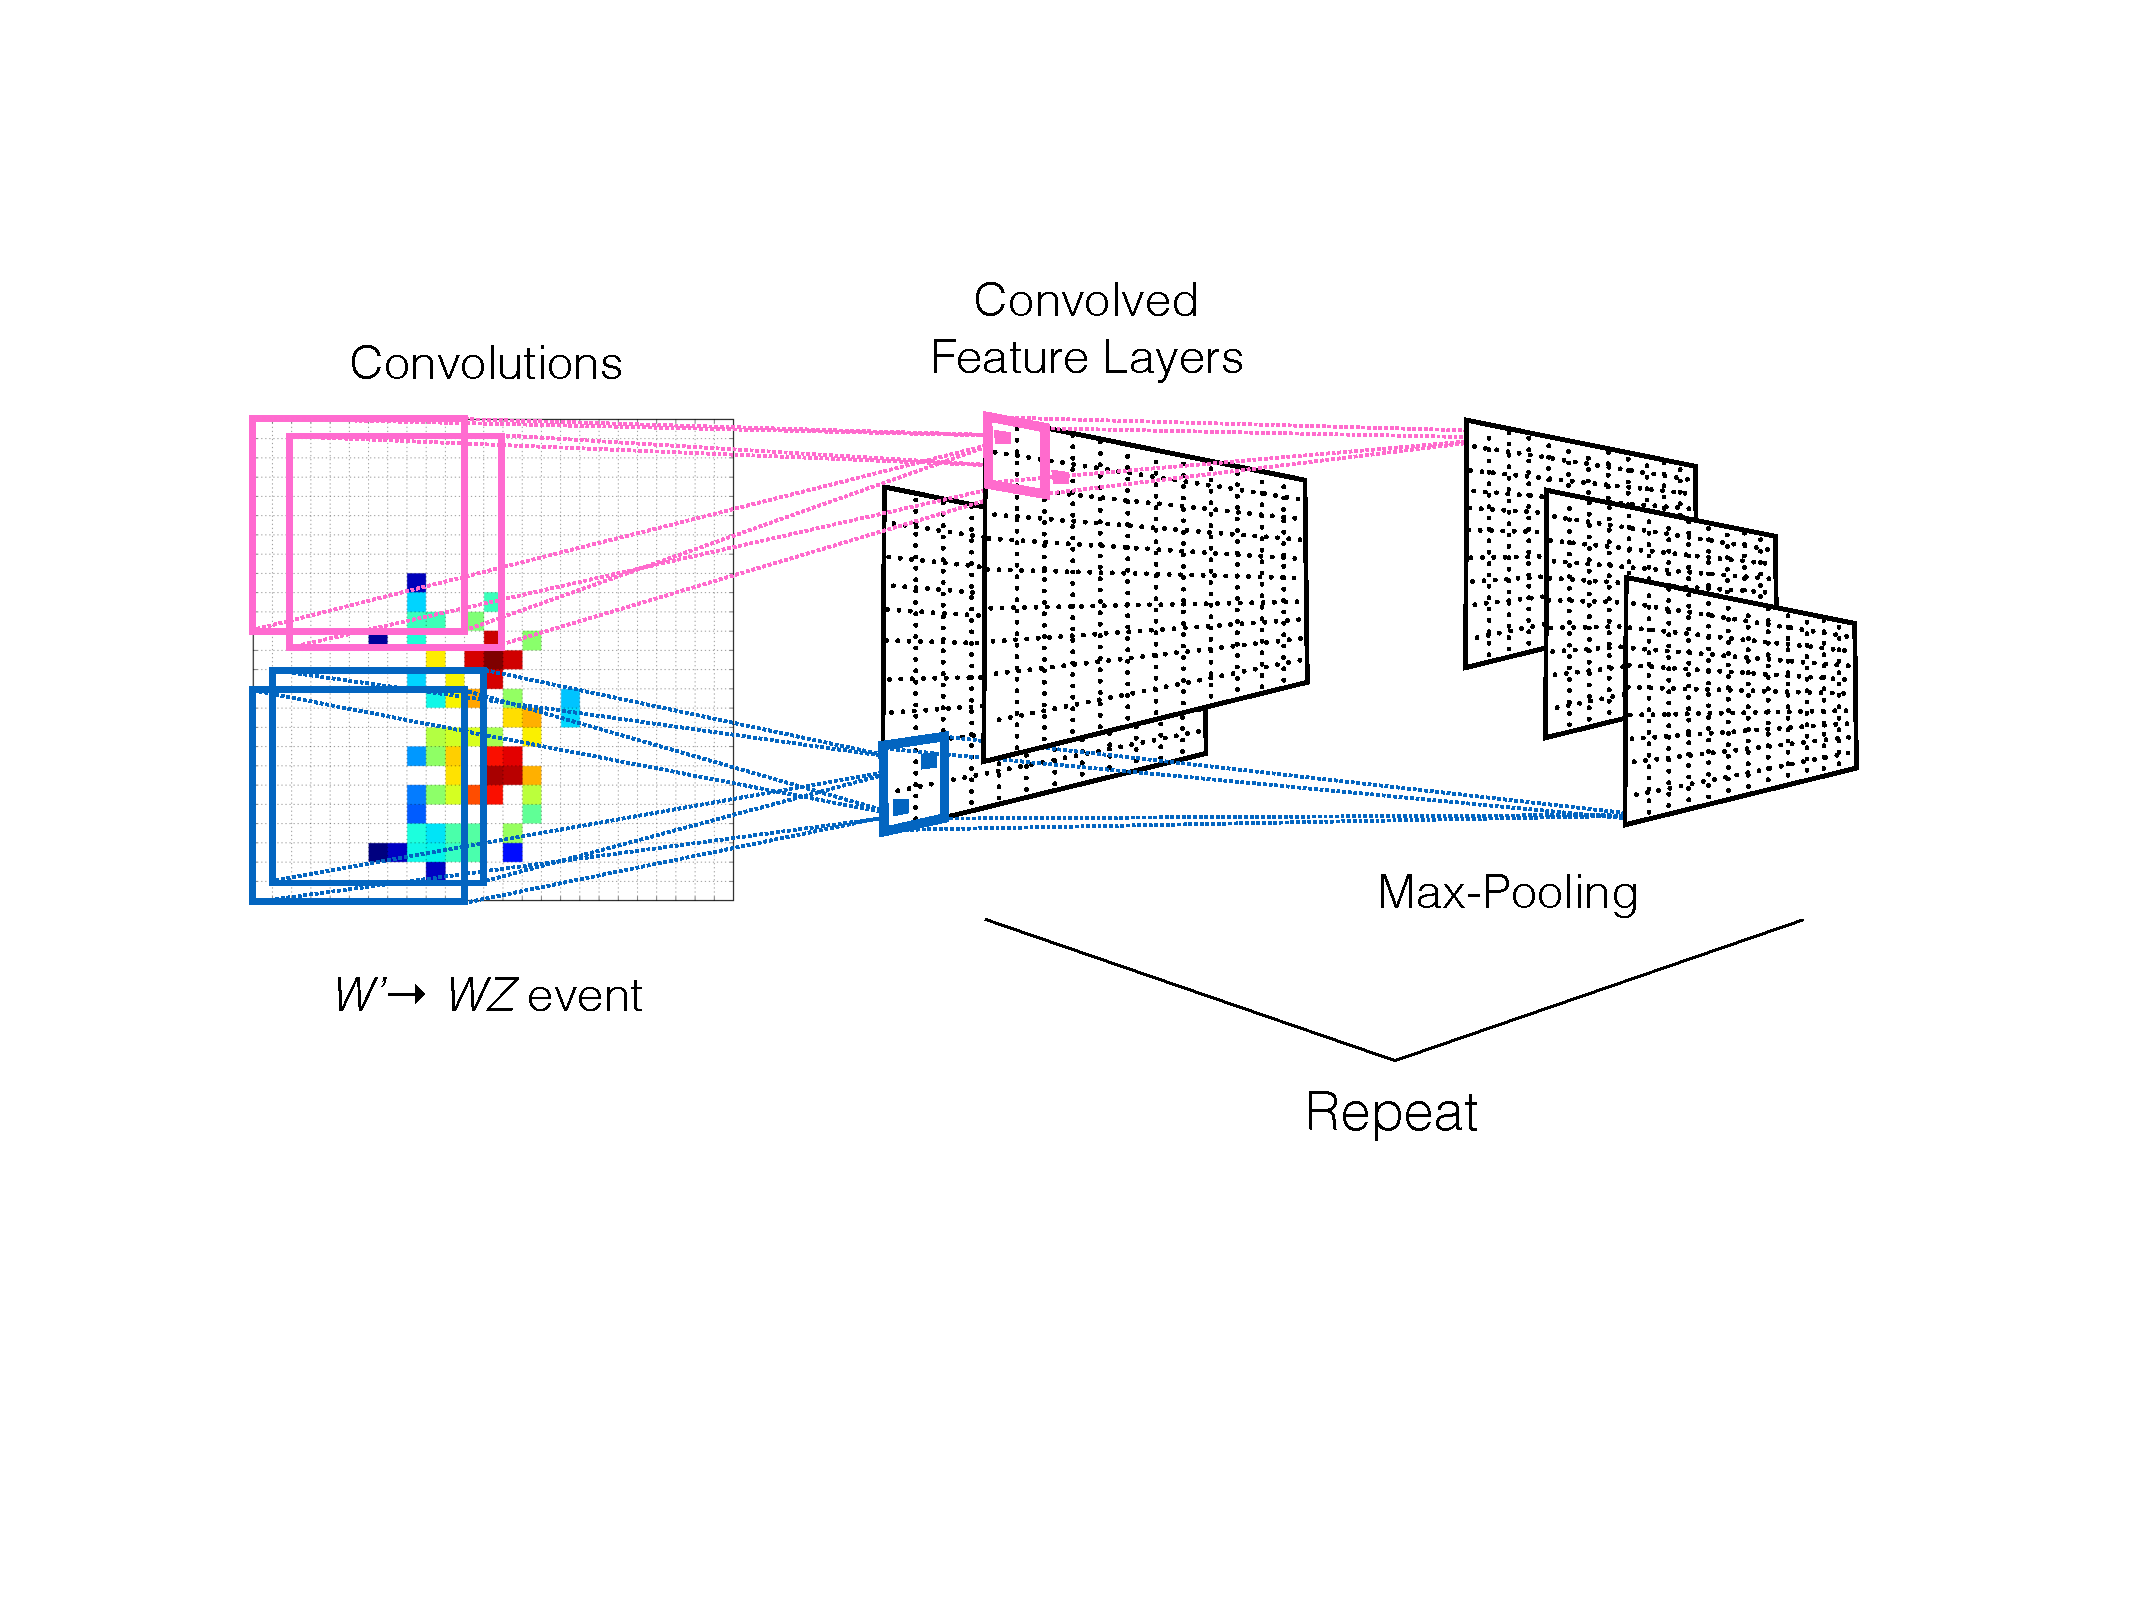
\includegraphics[width=0.75\textwidth]{figures/architecture.pdf}
  \caption{The convolution neural network concept as applied to jet-images.}
  \label{fig:arch}
\end{figure}

The convolution layers each utilize 32 feature maps, or filters, with filter sizes of $11\times 11$, $3\times 3$, and $3\times 3$ respectively.  All convolution layers are regularized with the $L^{2}$ weight matrix norm.  A down-sampling of $(2, 2)$, $(3, 3)$, and $(3, 3)$ is performed by the three max pooling layers, respectively.  A dropout~\cite{dropout:and:LRN} of 20\% is used before the first FC layer, and a dropout 10\% is used before the output layer.  The FC hidden layer consists of 64 units.

After early experiments with the standard $3\times 3$ filter size, we discovered significantly worse performance over a more basic MaxOut \cite{maxout:goodfellow} feedforward network. After further investigation into larger convolutional filter size, we discovered that larger-than-normal filters work well on our application. Though not common in the Deep Learning community, we hypothesize that this larger filter size is helpful when dealing with sparse structures in the input images. In Table~\ref{tab:kernelsize}, we show the optimal filter size of $11\times11$ while considering the metric outlined in Section~\ref{sec:studies}.

\begin{table}[h!]
  \centering
  \begin{tabular}{r|c}
    \bfseries Kernel size & \bfseries AUC \\ 
    \hline
    $(3 \times 3)$ Conv & 14.770 \\
    \hline
    $(4 \times 4)$ Conv & 12.452 \\
    \hline
    $(5 \times 5)$ Conv & 11.061 \\
    \hline
    $(7 \times 7)$ Conv & 13.308 \\
    \hline
    $(9 \times 9)$ Conv & 17.291 \\
    \hline
    $(11 \times 11)$ Conv & 20.286 \\
    \hline
    $(15 \times 15)$ Conv & 18.140 \\
  \end{tabular}
  \caption{First layer convolution size vs. performance}
  \label{tab:kernelsize}
\end{table}
% table

Two convolution networks, which differ in their pre-processing, are studied in this paper.  The first, which we refer to as the ConvNet, is trained (and evaluated) on un-normalized jet-images using the transverse energy for the pixel intensities.  The second, which we refer to as ConvNet-Norm, is trained (and evaluated) on $L^{2}$ normalized jet-images using the transverse-energy for the pixel intensities.  Examining the performance of both networks allows us to study the possible effects of the pre-processing.



% subsubsection architectural_selection (end)

\subsection{Implementation and Training} % (fold)
\label{ssub:implementation_and_training}

All Deep Learning experiments were conducted in Python with the Keras~\cite{Keras} Deep Learning library, utilizing NVIDIA C2070 graphics cards. One GPU was used per training, but several architectures were trained in parallel on different GPU's to optimize the performance of networks with different hyper-parameters.

We used 8 million training examples, with an additional 2 million validation samples for tuning the hyper-parameters, and 3 million testing samples.  Signal examples are weighted such that the total sum of weights is the same as the total number of background examples (as explained in Section~\ref{sec:simulation}).  These weights are used in the by the cost function in the training.  The networks were trained with the Adam~\cite{DBLP:journals/corr/KingmaB14} algorithm (Stochastic Gradient Descent with Nesterov Momentum~\cite{Nesterov:1983wy} was also examined, but did not provide performance gains).  The training consisted of 100 epochs, with a 10 epoch patience parameter on the increase in AUC between 0.2 and 0.8 on a validation set.  Batch sizes of 32 were used for the MaxOut network, while batch sizes of 96 were used for the convolution networks.

% subsubsection implementation_and_training (end)



\section{Studies} % (fold)
\label{sec:studies}

%%%%%%%%%%%
%%%    studies intro
%%%%%%%%%%%

In this section, we examine the performance of the MaxOut and Convolution deep neural networks, described in Section~\ref{sec:arch}, in classifying $W^\pm \to q q^\prime$ from QCD jets.  As one of our primary goals is to understand  what these NN's can learn about jet topology for discrimination, we focus on a restricted phase space of the mass and transverse momentum of the jets.  In particular, we restrict our studies to $250$ GeV $\leq p_T \leq 300$ GeV, and confine ourselves to a $65$ GeV $\leq m \leq 95$ GeV mass window, wholly containing the peak of the $W$.   We then construct a scaffolded and multi-approach series of methodologies for understanding, visualizing, and validating neural networks within HEP.

The figures of merit...


The performance evaluation and information exploration techniques are examined in three settings, all of which require the aforementioned mass and transverse momentum selection.
\begin{itemize}

\item \textbf{General Phase Space:} No alterations are made to the phase space.  This give an overview of the performance and information learned by the networks

\item  \textbf{Uniform Phase Space:}  The weights of each jet is altered such that the joint distributions of mass, $n$-subjettiness, and $p_T$ are non-discriminative.  Specifically, we derive weights such that:
\begin{equation}
  f(m, \tau_{21}, p_T| W'\rightarrow WZ) \approx f(m, \tau_{21}, p_T| QCD).
\end{equation}
Both thre reweighting and network evaluation are performed in slightly more restricted phase space requiring $\tau_{21}\in [0.2, 0.8]$. While $p_T$ is reweighted in all phase space setting, mass and $n$-subjettiness are also weighted in the setting as they are amongst the most discriminating physics-inspired variables.  This weighting ensures that mass, $n$-subjettiness, and $p_T$ do not contribute to differences between signal and background, and thus this information is essentially removed from the discrimination power of the networks.  This allows us to examine what information beyond these variables has been learned and to understand where the neural network performance improvements beyond these physics derived variables comes from.  Neural networks that are trained in the General Phase Space are applied as the discriminant under this ``flattening'' transformation. We also use the training weights inside this window and train an additional CNN. In particular, we look for increases in performance, which would indicate information learned beyond physics variables since we removed the discrimination power using this uniform weighting scheme.

\item \textbf{Highly Restricted Phase Space:} The phase space of mass, $n$-subjettiness, and $p_T$ are restricted to very small windows of size: $m\in [79, 81]$ GeV,  $p_T \in [250, 255]$ GeV, and  $\tau_21 \in [0.19, 0.21]$. No reweighting is performed, and the networks trained in the General Phase Space are used for discrimination and evaluation.  This highly restricted window is provides a different method to effectively remove any discrimination power of mass, $n$-subjettiness, and $p_T$ as there is little to no variation of the variables in these small windows for either signal or background.  Thus, any discrimination improvements of the neural networks over the physics-inspired variables would be coming from information learned beyond these variables.  While the reweighting in the Uniform  Phase Space is designed also to remove such discrimination, it produces a non-physical phase space.  Thus the Highly Restricted Phase Space allows us to be sure that the neural network performance improvements are valid and carry over to a less contrived phase space.

\end{itemize}
By examining the performance of the neural networks in these different phase spaces, we aim to systematically remove known discriminative information from the networks' performance and thereby probe the information learned beyond what is already known by physics inspired variables.

%To begin understanding what a deep network can learn about jet topology, we choose a finite region of phase space, and standardize our comparisons. In an effort to define a standard way that physics object identification using machine learning should be conducted, we exactly define our procedure for comparisons. 

\subsection{Figure of Merit} % (fold)
\label{sec:figure_of_merit}

As is commonly done in High Energy Physics, we eschew the commonly chosen metric of basic accuracy in favor of the Receiver Operating characteristic. This is because we must examine the entire spectrum of trade-off between Type-I and Type-II error, as many applications in physics will choose different points along the trade-off curve. We use a slight modification of the traditional ROC. For any discriminating variable, let $c$ be a threshold on the likelihood ratio on that variable, and let $w$ be the vector of weights over the entire evaluation sample. We define the \emph{rejection} of such a threshold is defined as 
$$
    \rho(c) = \frac{1}{\text{FPR}(c, w)},
$$
where $\text{FPR}(c, w)$ is the weighted false positive rate for using $c$ as a threshold.

We define the \emph{efficiency} of $c$ as 
$$
    \varepsilon(c) = \text{TPR}(c, w),
$$
where $\text{TPR}(c, w)$ is the weighted false positive rate for using $c$ as a threshold. We then evaluate our algorithms using the area under the line generated by $\{(\varepsilon(c), \rho(c)) : \varepsilon(c)\in [0.2, 0.8]\}$. We say that an classifier is \emph{strictly} more performant if the ROC curve is above a baseline for all efficiencies.


\subsection{Studies in the General Phase Space} % (fold)
\label{sub:coarse_studies}

In order to examine the overall discrimination performance of the DNN's to that of the physics-driven variables, we examine the ROC curves in Figure~\ref{fig:combinedROC1}. In particular, we compare the DNN's to $n$-subjettiness~\cite{nsub} $\tau_{21} = \tau_{2}/\tau_{1}$, the jet mass, and the distance $\Delta R$ between the leading two $p_{T}$ subjets.  In Figure~\ref{fig:combinedROC1a}, we can see that the three DNN's have similar performance, but the MaxOut networks tends to outperform the ConvNet networks.  We suspect that the MaxOut tends to outperform the ConvNets due to sparsity of the jet-images, whereby the MaxOut network views the full jet-image from the inital hidden layer while the sparsity tends to make it difficult for the ConvNets to learn meaningful convolution filters .  We also see that the ConvNet-Norm tends to outperform the ConvNet trained on the un-normalized jet-images.  As we will see soon,  it is difficult for these networks to fully learn the jet mass and thus the loss of mass information from normalization and energy  binning (rather than transverse energy) of the ConvNet-Norm training tends to not to impede performance.   Finally, we can see the Fisher-Jet discriminant\footnote{The Fisher discriminant is trained in three partitions of $\Delta  R$ ($\Delta R \in [0.25, 0.5],\ [0.5, 0.75],\ [>0.75])$, in order to account for the non-linear variation in jet-images from the differing positions of the two subjets.  Also note that unlike in the original implementation, here we do not normalize the jet images when computing the Fisher Jet.  This leads to slightly better performance.} performance, as described in reference~\cite{Cogan:2014oua}, which outperforms the physics inspired variables (as expected) but is much less performant than the DNN's. In addition, in Figure~\ref{fig:combinedROC1b} we see that the DNN's also outperform the two-variable combinations of the physics inspired variables (computed using the 2D likelihood ratio).   It is interesting to note that combining mass and $\tau_{21}$, or $\tau_{21}$ and $\Delta R$, achieve much higher performance than the individual variables and are significantly closer to the performance of the DNN's.  However, the large difference in performance between the DNN's and the physics-variable combinations implies the DNN's may be learning information that is not \emph{fully} encapsulated in these physics variables.
%This is likely due to the normalization and energy binning helping to provide more uniformity in the typical pixel intensities across jet-images.
\begin{figure}[!htbp]
\begin{center}
\subfloat[]{
	\includegraphics[width=0.48\textwidth,angle=0]{figures/ROC_1}
	\label{fig:combinedROC1a}
}
\subfloat[]{
	\includegraphics[width=0.48\textwidth,angle=0]{figures/ROC_2}
	\label{fig:combinedROC1b}
}
\end{center}
   \caption{Receiver Operating Characteristic (ROC) over coarse sample}
  \label{fig:combinedROC1}
\end{figure}


While we can see in Figure~\ref{fig:combinedROC1} that the DNN's outperform the individual and two-variable physics inspired discriminators, we want to understand if these physics variables have been learned by the networks.  As such, we compute the combination of the DNN's with each of the physics inspired variables (using the 2D likelihood), as seen for the ConvNet in Figure~\ref{fig:combinedROC2a} and for the MaxOut network in Figure~\ref{fig:combinedROC2b}. In both cases, we see that the discriminators combining $\Delta R$ or $\tau_{21}$ with the DNN's does not improve performance.  This indicate that the information contained in these physics-inspired variables  has already been fully learned by the networks.  However, adding mass in combination with the DNN's shows a noticeable improvement in performance over the DNN's alone.  This indicates that all of the information contained in the mass variable has not been learned by the DNN's.  While it is not shown, similar patterns are found for the Conv-Norm network.
\begin{figure}[!htbp]
  \begin{center}
\subfloat[]{
	\includegraphics[width=0.48\textwidth,angle=0]{figures/ROC_3}
	\label{fig:combinedROC2a}
}
\subfloat[]{
	\includegraphics[width=0.48\textwidth,angle=0]{figures/ROC_4}
	\label{fig:combinedROC2b}
}
\end{center}
  \caption{Receiver Operating Characteristic (ROC) over coarse sample}
  \label{fig:combinedROC2}
\end{figure}

Another way to inspect what information about the physics-inspired variables has been learned by the DNN's is to study the correlation between the DNN output and the physics-variables.  The correlations are shown in Figure~\ref{fig:sculptedConv} for the ConvNet, and in Figure~\ref{fig:sculptedConv} for the MaxOut network,  against the jet mass, $\Delta R$, and $\tau_{21}$.   These distributions are normalized in bins of the DNN output, and thus the $z$-axis is showing the probability of the physics variable given the network output (i.e. $P($variable | network output$)$). Normalizing the distributions in this way allows us to see the most probable values of the physics variables at each point of the network output, without being affected by the overall distribution of jets in this 2D space.  We can see that both networks show a strong (non-linear) correlations with $\tau_{21}$ and $\Delta R$, giving further evidence that this information has been learned by the networks.  However, the correlations are much weaker with the jet mass variable, being slightly more strongly correlated with the MaxOut network output.  While it is not shown, similar patterns are found for the Conv-Norm network.
\begin{figure}[htbp!]
  \begin{center}
  
  \subfloat[Sculpted QCD  ConvNet network output versus mass (left), $\Delta R$ (middle), and $\tau_{21}$ (right) distributions\label{fig:sculptedConv}]
      {
        \includegraphics[width=0.32\textwidth]{figures/mass_convnet_back_norm_invert.pdf}
         \includegraphics[width=0.32\textwidth]{figures/dR_convnet_back_norm_invert.pdf} 
         \includegraphics[width=0.32\textwidth]{figures/tau21_convnet_back_norm_invert.pdf}
      }\\
        \subfloat[Sculpted QCD  MaxOut network output versus mass (left), $\Delta R$ (middle), and $\tau_{21}$ (right) distributions\label{fig:sculptedMax}]
      {
        \includegraphics[width=0.32\textwidth]{figures/mass_maxout_back_norm_invert.pdf}
         \includegraphics[width=0.32\textwidth]{figures/dR_maxout_back_norm_invert.pdf} 
         \includegraphics[width=0.32\textwidth]{figures/tau21_maxout_back_norm_invert.pdf}
      }\\

      \caption{Sculpted QCD distributions}
      \label{fig:qcdsculpt}

    \end{center}
\end{figure}

\subsubsection{Understanding what is learned} % (fold)
\label{ssub:understanding_what_is_learned}

Though important on it's own, the ROC curves only begin to help us understand what information has been learned. The increased performance of the DNN's over the physics inspired variables and their combinations begs further questions: what is this gain, and where does it come from? Why is the DNN able to pick up on this? In order to improve our understanding of what we learn, we first take a look \emph{inside} the deep network, and visualize features learned during training.


In Figure~\ref{subfig:filters}, we show the first layer 11$\times$11 convolutional filters learned by our Conv-Norm network. Each filter is visualized by showing the learned weight in each position of the filter.  We can see that there is variation between filters, indicating that they are learning different features of the jet-images, but this variation is not as large as seen in many CV problems due to the sparsity of the jet-images.  We also see that they tend to learn representations of the subjets and distances between subjets, as seen by the circular features found in many of the filters.

To get a better understanding of how these filters provide discrimination, we mimic the operation in the first layer of the network by convolving each filter with average of large samples of signal and background jet images.  The difference between the average signal and average convolved background jet-images help to provide an understanding of what difference in features the network learns at the first layer in order to help discriminate.

More formally, let $J_s=\frac{1}{n}\sum_{i:i\text{ is signal}} J^{(i)}$ and $J_b=\frac{1}{n}\sum_{i:i\text{ is background}}J^{(i)}$ represent the average signal and background jet over a sample, where $J^{(i)}$ is the $i$th jet image. In addition, we can select a filter $w_i\in\mathbb{R}^{11\times11}$ from the first convolutional layer. We then examine the differences in the post convolution layer by computing:
\begin{equation}
  J_s \ast w_i - J_b \ast w_i, \forall i,
\end{equation}

where $\ast$ is the convolution operator. We arrange these new ``convolved jet-images'' in a grid, and show in red regions where signal has a stronger representation, and in blue where background has a stronger representation. In Figure~\ref{subfig:convolvedfilters}, we show the convolved differences described above, where each $(i, j)$ image is the representation under the $(i, j)$ convolutional filter. We note the existence of interesting patterns around the regions where the leading and subleading subjets are expected to be. We also draw attention to the fact that there is a large diversity in the the convolved representations, indicating that the DNN is able to learn and pick up on multiple features that are descriptive.
\begin{figure}[bt]
  \begin{center}
      \subfloat[$(11\times11)$ convolutional kernels from first layer \label{subfig:filters}]{
        \includegraphics[width=0.5\textwidth]{figures/conv-filts.pdf}
      }
      \subfloat[Convolved Jet Image differences\label{subfig:convolvedfilters}]{
        \includegraphics[width=0.5\textwidth]{figures/conv-diffs-global.pdf}
      }
      \caption{Convolutional Kernels (left), and convolved feature differences in jet images (right)}
      \label{fig:convkernels}

    \end{center}
\end{figure}



\subsubsection{Physics in Deep Representations} % (fold)
\label{ssub:physics_in_deep_representations}
To get a tangible and more intuitive understanding of what jet structures a DNN learns, we compute the correlation of the Conv-Norm network output with each pixel of the jet-images. Specifically, let $y$ be the DNN output, and consider every pixel $p_ij$ in transformed $(\eta, \phi)$ space. We the construct an image, which we denote the \emph{deep correlation jet-image}, where each pixel $(i, j)$ is $\rho_{p_{ij}, y}$, the Pearson Correlation Coefficient of that pixels energy deposition with the final DNN output. While this this image does not give a direct view of the discriminating information learned within the network, it does provide a guide to how such information may be contained within the network.  In Figure~\ref{fig:corr}, we construct this deep correlation jet-image, and can see a wealth of interesting structure.  We can see that the location and energy of the subleading subjet, found at the bottom of the image, is highly correlated with the DNN output and important for identifying signal jet-images.  In contrast, the information contained in the leading subjet, seen at $(x,y)\sim (0,0)$ in the image, is not particularly correlated with the network owing to the fact that both signal and background jets have high energy leading subjets.  We also see asymmetric regions around both subjets that are correlated with the DNN output and is likely indicating the presence of additional radiation expected in the QCD background jets.  Finally, a small negative correlation with the rest of the jet area is seen, indicating that radiation from the background jets is more likely to be observed in these regions.   The exact function form of this distribution is not known, nor does it seem to describe exactly any known physics inspired variable.
\begin{figure}[!htbp]
  \centering
  \includegraphics[width=0.5\textwidth]{figures/pixel-activations-corr.pdf}
  \caption{Per-pixel linear correlation with DNN output}
  \label{fig:corr}
\end{figure}


\clearpage

\subsection{Studies in the Uniform Phase Space} % (fold)
\label{sub:flat_hypercube_studies}

Since we outperform physics-derived variables, we would like to know where these performance improvements come from. Our first approach to this is \emph{hypercube reweighting}. In particular, we derive weights such that the joint distributions of mass, $n$-subjettiness, and $p_T$ are non-discriminative. Specifically, we require

\begin{equation}
  f(m, \tau_{21}, p_T| W'\rightarrow WZ) \approx f(m, \tau_{21}, p_T| QCD).
\end{equation}

We then take our globally trained neural network (Figure~\ref{fig:combinedROC}) and apply the discriminant under this ``flattening'' transformation. We also use the training weights inside this window and train an additional CNN. In particular, we look for increases in performance, which would indicate information learned beyond physics variables since we removed the discrimination power using hypercube weighting.

In Figure~\ref{fig:rocCube} we show that the globally trained NN retains discrimination power even once we ``subtract'' the discrimination power of primitives from physics.

\begin{figure}[htbp]
  \centering
  \includegraphics[width=0.95\textwidth]{figures/roc-cube-inside.pdf}
  \caption{ROC Curve for weigth-flattened hypercube, with $m\in[65, 95]\mathsf{GeV}$,  $p_T\in[250, 300]\mathsf{GeV}$, and  $\tau_{21}\in[0.2, 0.8]$}
  \label{fig:rocCube}
\end{figure}

% subsection flat_hypercube_studies (end)
\clearpage

\subsection{Studies in the Highly Restricted Phase Space} % (fold)
\label{sub:small_window_studies}

Removing the discrimination power of $\tau_{21}$ and the jet mass in Sec.~\ref{sub:flat_hypercube_studies} allowed us to quantify the unique discrimination power learned by the neural networks.  However, it does not tell us what information is learned.  Another way to quantify the unique information learned by the network that also provides useful information about physical information learned by the network is to restrict the considered phase space such that $\tau_{21}$ and the jet mass distributions do not vary appreciably over the redacted space.  Figure~\ref{fig:meanImagesWindow} shows the average signal and background jet image in three small windows of $\tau_{21}$, the jet mass, and the jet $p_T$.  In all three windows, the jet mass is restricted to be between 79 GeV and 81 GeV and the jet $p_T$ is required to be in the interval [250,260] GeV.  The three windows are then defined by their value of $\tau_{21}$: [0.19,0.21] in the most two-prong-like case, [0.39,0.41] in a region with likelihood ratio near unity and [0.59,0.61] in a mostly one-prong-like case.  The key physics features of the jets falling in these windows are easily visualized from the average jet images.  The most striking observation is that in these three windows, signal jets look very similar to background jets.  When $\tau_{21}\in[0.19,0.21]$, both signal and background jets have a second subjet that is distinct from the leading subjet and this is washed out as the value of $\tau_{21}$ increases.  

The differences between images in these small windows tells us about what information {\it could be learned} by the networks beyond $\tau_{21}$ and the jet mass.  Since the differences are subtle, the average difference is explicitly computed and plotted in Fig.~\ref{fig:meanImagesWindow2} for the three narrow windows of $\tau_{21}$.  In the window with $\tau_{21}\in[0.19,0.21], there are five features: a localized blue patch in the bottom center, a localized red patch just above that, a red diffuse region between the red patch and the center and then a blue dot just left of center surrounded by a red shell to the right.  Each of these have a physics meaning: the lower two localized patches give information about the orientation of the second subjet $(\Delta R)$ which is slightly wider for the QCD jets which need a slightly wider angle to satisfy the mass requirement.  The red diffuse region just above the localized patches is likely an indication of colorflow: the $W$ bosons are color singlets compared to the color octet gluon jet background, and thus we expect the radiation pattern to be mostly between the two subjets for the $W$.  There is a similar story for all the features in each of the plots in Fig.~\ref{fig:meanImagesWindow2}.

\begin{figure}[bt]
  \begin{center}
  
        \includegraphics[width=0.99\textwidth]{figures/averages_fixed_nonorm.pdf}

      \caption{
        $W'\rightarrow WZ$ (top) and QCD (bottom) average jet-images in three small windows of $\tau_{21}$: [0.19, 0.21] (left), [0.39, 0.41] (middle), and [0.59, 0.61] (right).  In all cases, jet mass is restricted to be between 79 GeV and 81 GeV and the jet $p_T$ is required to be in the interval [250,260] GeV.
        \label{fig:meanImagesWindow} 
      }
    \end{center}
\end{figure}  

\begin{figure}[bt]
  \begin{center}
  
        \includegraphics[width=0.99\textwidth]{figures/difference_fixed_nonorm.pdf}
        
      \caption{
         The average difference between $W'\rightarrow WZ$ jet-images in three small windows of $\tau_{21}$: [0.19, 0.21] (left), [0.39, 0.41] (middle), and [0.59, 0.61] (right).  In all cases, jet mass is restricted to be between 79 GeV and 81 GeV and the jet $p_T$ is required to be in the interval [250,260] GeV.  The red colors are more signal-like and the blue is more background-like.
        \label{fig:meanImagesWindow2} 
      }
    \end{center}
\end{figure}  

\begin{figure}[htbp]
  \centering
  \includegraphics[width=0.5\textwidth]{figures/augwindow-roc.pdf}
  \caption{Receiver Operating Characteristic (ROC) over window sample}
  \label{fig:rocWindow}
\end{figure}

%\subsubsection{Understanding what we learn} % (fold)
%\label{ssub:understanding_what_we_learn}

Now, we turn back to the neutral network and their performance in these small windows of jet mass and $\tau_{21}$.    Figure~\ref{fig:rocWindow} shows three ROC curves in the window $\tau_{21} \in[0.19,0.21].  By construction, the $\tau_{21}$ curve is no better than a random guess, since this variable does not significantly vary over the small window.  The other two curves are a Fisher Linear Discriminant\footnote{There is no $\Delta R$ binning as in the Fisher Jets of Ref.~\cite{Cogan:2014oua}, but this will make little difference since the $\Delta R$ distribution does not significantly compared with the coarse $\Delta R$ bins within the small mass and $p_T$ windows.} (FLD)

In this window, we compare the DNN trained outside the window to a Fisher Linear Discriminant trained inside the window. In Figure~\ref{fig:rocWindow} we see this performance comparison, and note that our DNN outperforms the FLD.

\begin{figure}[htbp]
  \centering
  \includegraphics[width=0.65\textwidth]{figures/fld-benwindow.pdf}
  \caption{Cell coefficients from Fisher Linear Discriminant in window: $m_\text{jet}\in [79, 81]$ GeV, $p_{T}\in [250, 255]$ GeV, $\tau_{21}\in[0.19, 0.21]$}
  \label{fig:fldWindow}
\end{figure}

\begin{figure}[htbp]
  \centering
  \includegraphics[width=0.65\textwidth]{figures/pixel-activations-corr-benwindow.pdf}
  \caption{Pearson Correlation Coefficient for pixels vs. DNN output, $m_{\mathsf{jet}}\in [79, 81]$ GeV, $p_{T}\in [250, 255]$ GeV, $\tau_{21}\in[0.19, 0.21]$}
  \label{fig:corrWindow}
\end{figure}

%In Figure~\ref{fig:convkernelsWindow}, we show the same feature representations as in Figure~\ref{subfig:convolvedfilters}, which show the convolved differences in images over signal and background in the window. 
%
%\begin{figure}[htbp]
%  \centering
%  \includegraphics[width=0.95\textwidth]{figures/conv-diffs-ben-window.pdf}
%  \caption{Convolved Feature Differences in jet images, $m_\text{jet}\in [79, 81]$ GeV, $p_{T}\in [250, 255]$ GeV, $\tau_{21}\in[0.19, 0.21]$}
%  \label{fig:convkernelsWindow}
%\end{figure}


% subsubsection understanding_what_we_learn (end)

% subsection small_window_studies (end)




\clearpage
\newpage

% section studies (end)


\section{Acknowledgements} % (fold)
\label{sec:acknowledgements}

We would like to thank Andrew Larkoski for useful conversations about the physics observed in the jet images.  This work is supported by the Stanford Data Science Initiative and by the US Department of Energy (DOE) under grant DE-AC02-76SF00515. BN is supported by the NSF Graduate Research Fellowship under Grant No. DGE-4747 and by the Stanford Graduate Fellowship.  

% section acknowledgements (end)


% \nocite{*}
 \bibliography{myrefs}





\end{document}
